% !TeX spellcheck = cs_CZ
{\tikzset{external/prefix={tikz/FYZII/}}
 \tikzset{external/figure name/.add={ch31_}{}}
%---------------------------------------------------------------------------------------------------
% file fey2ch31.tex
%---------------------------------------------------------------------------------------------------
%=========================== Kapitola Tenzory ======================================================
\chapter{Tenzory}\label{fyz:IIchapXXXI}
\minitoc
  \section{Tenzory polarizovatelnosti}\label{fyz:IIchapXXXIsecI}
  \section{Transformace tenzorových složek}\label{fyz:IIchapXXXIsecII}
  \section{Elipsoid energie}\label{fyz:IIchapXXXIsecIII}
  \section{Jiné tenzory. Tenzor setrvačnosti}\label{fyz:IIchapXXXIsecIV}
  \section{Vektorový součin}\label{fyz:IIchapXXXIsecV}
  \section{Tenzor napětí}\label{fyz:IIchapXXXIsecVI}
  \section{Tenzory vyššího řádu}\label{fyz:IIchapXXXIsecVII}
  \section{Čtyřtenzor elektromagnetické energie a hybnosti}\label{fyz:IIchapXXXIsecVIII}
  \section{Příklady a cvičení}\label{fyz:IIchapXXXIsecIX}

    \begin{figure}[ht!]   %\ref{fyz_fig874}
      \centering
      \begin{tabular}{c}
        \subfloat[ ]{\label{fyz_fig874a}
          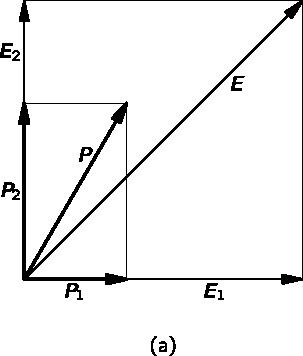
\includegraphics[width=0.7\linewidth]{fyz_fig874a.pdf}}               \\
        \subfloat[ ]{\label{fyz_fig874b}
          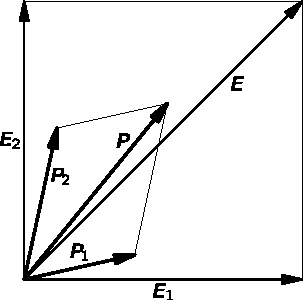
\includegraphics[width=0.7\linewidth]{fyz_fig874b.pdf}}
      \end{tabular}
      \caption{
               (\cite[s.~748]{Feynman02})}
      \label{fyz_fig874}
    \end{figure}

    \begin{figure}[ht!] %\ref{fyz_fig875}
      \centering
      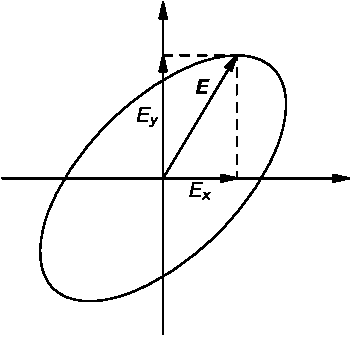
\includegraphics[width=0.7\linewidth]{fyz_fig875.pdf}
      \caption{
               (\cite[s.~707]{Feynman02})}
      \label{fyz_fig875}
    \end{figure}

    \begin{figure}[ht!] %\ref{fyz_fig876}
      \centering
      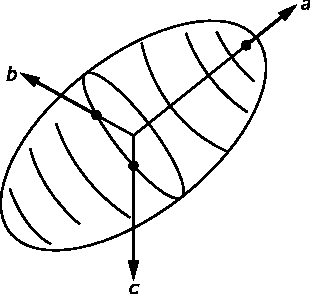
\includegraphics[width=0.7\linewidth]{fyz_fig876.pdf}
      \caption{
               (\cite[s.~707]{Feynman02})}
      \label{fyz_fig876}
    \end{figure}

    \begin{figure}[ht!] %\ref{fyz_fig877}
      \centering
      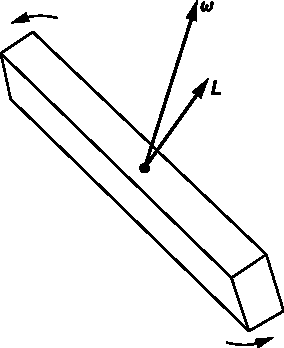
\includegraphics[width=0.7\linewidth]{fyz_fig877.pdf}
      \caption{
               (\cite[s.~707]{Feynman02})}
      \label{fyz_fig877}
    \end{figure}

    \begin{figure}[ht!] %\ref{fyz_fig878}
      \centering
      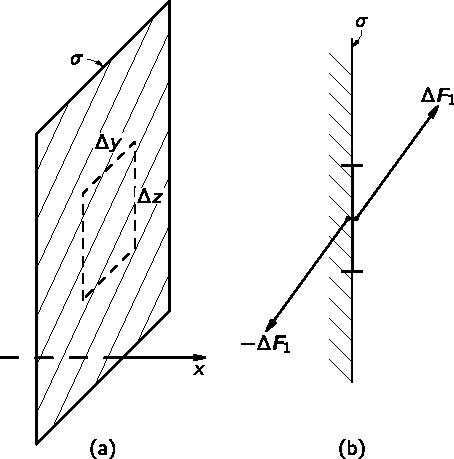
\includegraphics[width=0.7\linewidth]{fyz_fig878.pdf}
      \caption{
               (\cite[s.~707]{Feynman02})}
      \label{fyz_fig878}
    \end{figure}

    \begin{figure}[ht!] %\ref{fyz_fig879}
      \centering
      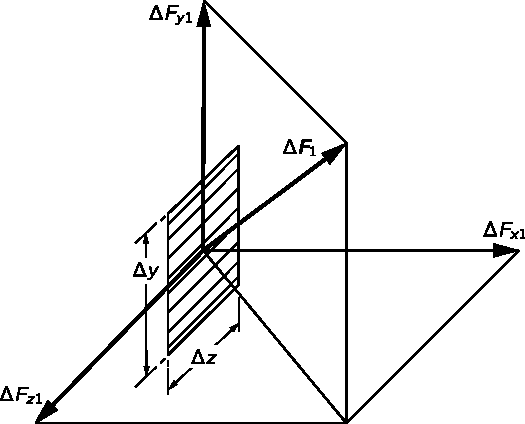
\includegraphics[width=0.7\linewidth]{fyz_fig879.pdf}
      \caption{
               (\cite[s.~707]{Feynman02})}
      \label{fyz_fig879}
    \end{figure}

    \begin{figure}[ht!] %\ref{fyz_fig880}
      \centering
      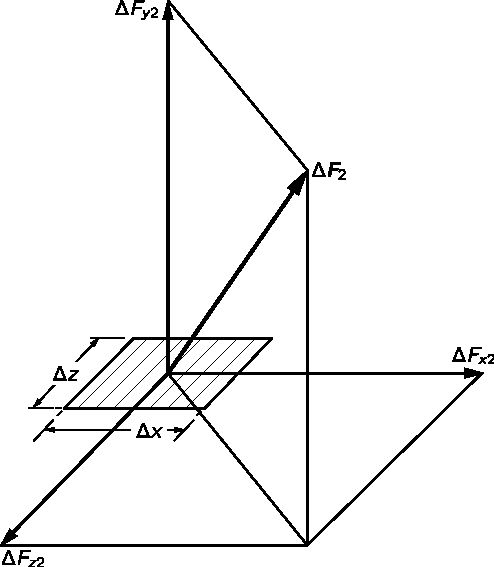
\includegraphics[width=0.7\linewidth]{fyz_fig880.pdf}
      \caption{
               (\cite[s.~707]{Feynman02})}
      \label{fyz_fig880}
    \end{figure}

    \begin{figure}[ht!] %\ref{fyz_fig881}
      \centering
      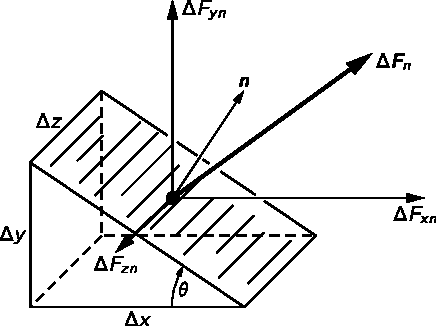
\includegraphics[width=0.7\linewidth]{fyz_fig881.pdf}
      \caption{
               (\cite[s.~707]{Feynman02})}
      \label{fyz_fig881}
    \end{figure}

    \begin{figure}[ht!] %\ref{fyz_fig882}
      \centering
      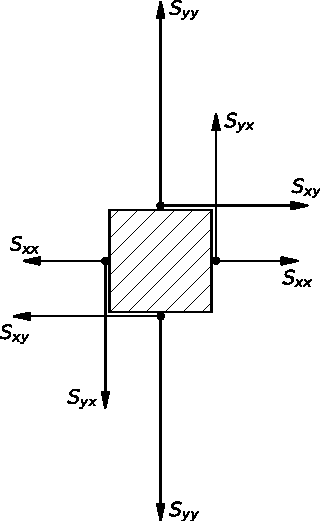
\includegraphics[width=0.7\linewidth]{fyz_fig882.pdf}
      \caption{
               (\cite[s.~707]{Feynman02})}
      \label{fyz_fig882}
    \end{figure}



} %tikzset
%---------------------------------------------------------------------------------------------------
\printbibliography[title={Seznam literatury},heading=subbibliography]
\addcontentsline{toc}{section}{Seznam literatury}